\subsection{Ковариация}

$$Cov(\xi,\eta) =E_{\xi \eta} -  E_{\xi}E_{\eta}$$

\deff{Ковариация} или \deff{корреляционный момент} показывает на сколько зависимы случайные величины это мера зависимости двух случайных величин.

Если $\xi, \eta$ - независимые случайные величины
$$Cov(\xi,\eta) = 0$$
$$Cov(\xi,\xi) = D_\xi = Var_\xi \text{ - вариация}$$

\subsection{Корреляция}

$$Corr(\xi,\eta) =\cfrac{E_{\xi \eta} -  E_{\xi}E_{\eta}}{\sqrt{D_{\xi}\cdot D_{\eta}}} = \cfrac{Cov(\xi,\eta)}{\sqrt{D_{\xi}\cdot D_{\eta}}}$$

\deff{Корреляция} - статистическая взаимосвязь двух случайных величин. Корреляция является \textbf{нормированной} версией ковариации, что позволяет сравнивать силу линейной зависимости между различными парами переменных, независимо от их масштаба.

\thmm{Теорема (об ограниченности корреляции)}
$$-1\leq Cor(\xi,\eta)\leq 1$$
\textbf{Доказательство:}

Возьму $\alpha = \xi - \lambda \eta$:
$$D\alpha = D(\alpha) = E\xi^2 - 2\lambda E_{\xi\eta} + \lambda^2E \eta^2-(E\xi)^2 + 2\lambda E_{\xi}E_{\eta}-\lambda^2(E_\eta)^2\geq 0$$
$$D\xi - 2\lambda Cov(\xi,\eta) + \lambda^2 D\xi \geq 0$$
Откуда, если рассматривать это, как уравнение относительно $\lambda$, то $D\leq 0 $, то есть:
$$4Cov(\xi,\eta) - 4 D_{\eta}D_{\xi}\leq 0$$
А если присмотреться, то это и есть то, что нам надо.

\hfill Q.E.D.

\subsection{Хвостовые неравенства}

Рассмотрим азартную игру. \sout{не одобряем, не играем.} 

Проводится случайный эксперимент, смотрится значение $\xi$. Если оно получилось 100 или больше, то мы платим 100 рублей, а иначе наш друг платит нам 100 рублей. Мы знаем $ E\xi = 10, \xi\geq 0$.

Хотим оценить $P(\xi\leq 100)$:
\begin{center}
    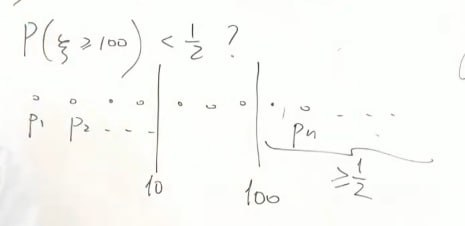
\includegraphics[width = 10cm]{assets/3_3_1.jpg}
\end{center}

Давайте посмотрим, является ли наша вероятность меньше $\frac 1 2$. Тогда всё, что правее 100 имеет вероятность выпадения $\geq \frac1 2 $. Все левое оценивается нулем, откуда мат ожидание хотя бы 50. Такого быть не может. В общем случае:

\thmm{Теорема (Неравенство Маркова)}
$$\xi\not \equiv0,\xi\geq 0: \forall a\geq 1: P(\xi\geq a \cdot E\xi) \leq \cfrac{1}{a}$$
\textbf{Доказательство:}
$$E_{\xi} = \sum\limits_{v}v \cdot P(\xi = v) = \sum\limits_{v < a \cdot E\xi} v P(\xi = v)+ \sum\limits_{v\geq a\cdot E\xi} v P(\xi=v)\geq \sum\limits_{v\geq a\cdot E\xi} a E{\xi} P(\xi=v) = a E{\xi}\cdot P (\xi\geq a\cdot E{\xi})$$
\hfill Q.E.D.

\thmm{Теорема (Неравенство Чебышева)} \\  \\
Абсолютная версия и относительная версия ($\alpha = \lambda\sigma$):
$$P(|\xi-E\xi|\geq \alpha)\leq \cfrac{D\xi}{\alpha^2} \quad \quad P(|\xi-E\xi|\geq \lambda\sigma)\leq \cfrac{1}{\lambda^2}$$
\textbf{Доказательство:}\\
Возьму вот такие величины:
$$D_{\xi} = E(\xi-E\xi)^2\quad \quad  \eta = (\xi-E\xi)^2$$
Заметим, что $E\eta=D\xi$. Используем неравенство Маркова для оценки дисперсии:
$$P(\eta\geq c*E\eta)\leq \cfrac{1}{c}$$
Возьму $c= \cfrac{D_{\xi}}{\alpha^2}$ и получу искомое

\hfill Q.E.D.

\textbf{Нечестная монета}. Вот вам дали домашку, вместе  с вопросом $p>\frac{1}{2}$ или $p<\frac{1}{2}$. Что вы можете делать? Только кидать ее, но при этом бесконечное количество раз вы не кинете, у вас дедлайн домашки через час. 

Пусть мы бросили $n$ раз. Выпало $c$ единиц и $n-c$ нулей. Пусть $c\le \frac{n}{2}$:
$$P(\xi = c)\leq P(\xi\leq c)\leq P(|\xi-pn|\geq pn-c)\leq  P(|\xi-pn|\geq \frac n 2 c)\leq \cfrac{n}{4}\cdot \cfrac{1}{\left(\cfrac{n}{2}-c\right)^2}$$
Что это концептуально значит? На самом деле то, это дает нам оценку на распределение. Зачем? Чтобы \textbf{\uline{СДАТЬ}} домашку.

\thmm{Теорема (Граница Чернова)}
$$P(\xi\geq (1+\varepsilon)p)\leq e^{-\frac{\varepsilon^2}{2+\varepsilon}np} \quad \Leftrightarrow\quad P(\xi\geq (1+\varepsilon)p)\leq e^{-\frac{\varepsilon^2}{2}np}$$
$$e^{-\frac{\varepsilon^2}{3}np}\leq \delta\quad \Leftrightarrow\quad -\dfrac{\varepsilon^2}{3}np\leq \ln{\delta}$$
$$n\geq \frac{3}{p\varepsilon^2}\ln{\frac{1}{\delta}}$$

Не знаю, что это концептуально, напишите пж